\chapter{\IfLanguageName{dutch}{Proof of Concept}{Proof of Concept}}%
\label{ch:proofOfConcept}

\section{Keuze van het proces}
\label{sec:keuze-proces}

In de interviews met de consultants van delaware kwamen meerdere processen naar boven die de werknemers zelf opgaven als processen uit hun dagelijkse werkleven die via RPA geautomatiseerd kunnen worden.
Deze processen worden hier nog eens opgelijst:

\begin{itemize}
    \item Lijst van Transport Requests tussen twee verschillende systemen controleren.
    \item Ophalen van systeem-gegevens voor een bepaalde klant.
    \item Verkooporders goedkeuren.
    \item Klantenservice voor betalingen en orders.
    \item Bestanden inlezen en automatisch soorteren aan de hand van AI en ML binnen RPA.
    \item CI/CD pipeline opzetten.
\end{itemize}

In Hoofdstuk~\ref{ch:stand-van-zaken} zijn er 3 belangrijke factoren gevonden die bepalen of een process geschikt is om geautomatiseerd te worden via RPA. Deze factoren zijn de frequentie waarmee het process uitgevoerd wordt, hoe complex het process is en of de verschillende stappen voldoende gestandardiseerd zijn.

In tabel \ref{tab:processen} worden de verschillende processen vergeleken ten opzicht van deze factoren en wordt er een score gegeven op 3. Hierbij is 3 de hoogste score, wat betekent dat het process aan de hand van deze factor zeer geschikt is om geautomatiseerd te worden. Een 1 daarentegen betekent dat het process voor deze factor minder geschikt is voor een automatisering.
Bij de factor 'frequentie' wordt er gekeken hoe vaak het proces wordt uitgevoerd. Een 3 betekent hier een veelvoorkomend process, een 1 betekent een process dat zelden voorkomt.
Bij de factor 'complexiteit' wordt er gekeken naar de verschillende stappen die ondernomen moeten worden en hoeveel applicaties er betrokken zijn. Een 3 betekent hierbij een relatief eenvoudig process, een 1 betekent een process met een verhoogde complexiteit.
Bij de factor 'gestandardiseerd' wordt er gekeken naar de verschillende stappen binnen het proces en of die wel of niet gestandardiseerd zijn en dus weinig variatie hebben. Een 3 betekent hierbij een proces met weinig afwijkingen, die vaak hetzelfde verloopt. Een 1 betekent een proces met veel variatie, die dus per uitvoering anders kan zijn.

\begin{table}[h]
    \centering
        \begin{tabular}{|l|l|l|l|l|}
            \hline
            Proces & Frequentie & Complexiteit & Gestand. & Totaal \\ \hline
            Transport Requests controleren & 3 & 3 & 3 & 9 \\ \hline
            Ophalen van systeem-gegevens & 2 & 2 & 3 & 7 \\ \hline
            Verkooporders goedkeuren & 3 & 2 & 1 & 6 \\ \hline
            Klantenservice voor betalingen & 2 & 2 & 2 & 6 \\ \hline
            Bestanden inlezen en sorteren & 2 & 2 & 2 & 6 \\ \hline
            Statement of Work aanmaken & 1 & 2 & 3 & 6 \\ \hline
            Powerpoint maken vanuit bestand & 2 & 2 & 1 & 5 \\ \hline
            CI/CD Pipeline opzetten & 1 & 1 & 1 & 3 \\ \hline
        \end{tabular}
    \caption{Vergelijking van de verschillende processen}
    \label{tab:processen}
\end{table}

Nu de processen vergeleken zijn, is het duidelijk dat er 1 proces erboven uitsteekt. Het proces 'Transport Requests controleren' is een proces dat dagelijks moet gebeuren, heel repetitief en eenvoudig is en weinig variatie heeft. Transport Requests worden gebruikt om aanpassingen binnen een systeem over te zetten naar een ander systeem. Wanneer deze niet op de juiste manier overgezet worden kunnen er stukken code overschreven worden of bepaalde afhankelijkheden niet mee overgezet worden, waardoor deze controle zeer cruciaal is. Dit maakt het dan ook een zeer geschikt proces om te automatiseren via RPA. Voor de Proof of Concept zal voor dit proces een RPA-automatisering gemaakt worden.

\section{Keuze van de RPA-software}
\label{sec:keuze-software}

Voor de keuze van de RPA-software zijn er meerdere opties. In Sectie~\ref{sec:verschillende-verdelers-van-rpa-software} werden verschillende RPA-verdelers onderzocht en vergeleken. Ook uit de interviews met de consultants van delaware kwamen een aantal verdelers naar boven. In de literatuurstudie werd besproken dat het belangrijk is om een RPA-verdeler te selecteren op basis van het proces en de kennis die een bedrijf al binnenshuis heeft.
Binnen delaware wordt er gesproken over 3 grote RPA-verdelers. Deze zijn UIPath, SAP BPA en Microsoft Power Automate. Aangezien het geselecteerde proces gebruikt maakt van een SAP-systeem, is het duidelijk dat UIPath en SAP BPA de meest geschikte keuzes zijn. Alhoewel Microsoft Power Automate ook een optie zou kunnen zijn, is deze zoals hierboven vermeld vooral geschrikt voor automatiseringen binnen een Microsoft omgeving.
Om een keuze te maken tussen UIPath en SAP BPA werd gekeken naar de algemene kennis binnen delaware. Binnen het automation team is UIPath zeer gekend, maar binnen het SAP Development team, het team waarvoor deze Proof of Concept wordt uitgewerkt, is deze kennis eerder beperkt en neigen ze meer naar SAP BPA. Dit is ook logisch, aangezien dit team werkt met SAP-producten.
Via deze redenering werd er voor deze Proof-of-Concept gekozen voor SAP BPA om de automatisering tot stand te brengen.

\section{Uitwerking Proof of Concept}
\label{sec:uitwerking-proof-of-concept}

Wanneer zowel het proces als de software gekozen is, werd de ontwikkeling van de automatisering gestart. Hiervoor werden de stappen die besproken werden in de literatuurstudie gevolgd.
De analyse en de procesevaluatie zijn reeds uitgevoerd in de vorige secties. Hieronder volgen de volgende stappen binnen het verloop van een RPA-project.

\subsection{Planning en design}
\label{subsec:planning-design}

Als eerste stap is het belangrijk om het proces in beeld te brengen. Hiervoor werd een flowchart opgezet die de verschillende stappen omschrijft die de bot zal moeten doorlopen om het proces tot een goed einde te brengen. Ook worden de uitzonderingen die voor kunnen komen gemapt in de flow.
Vanuit deze flowchart kan een ontwikkelaar dan de RPA-bot creëren.
De flowchart die voor dit proces werd opgesteld is te zien op afbeelding \ref{fig:flowchart}.

\begin{figure}
    \centering
    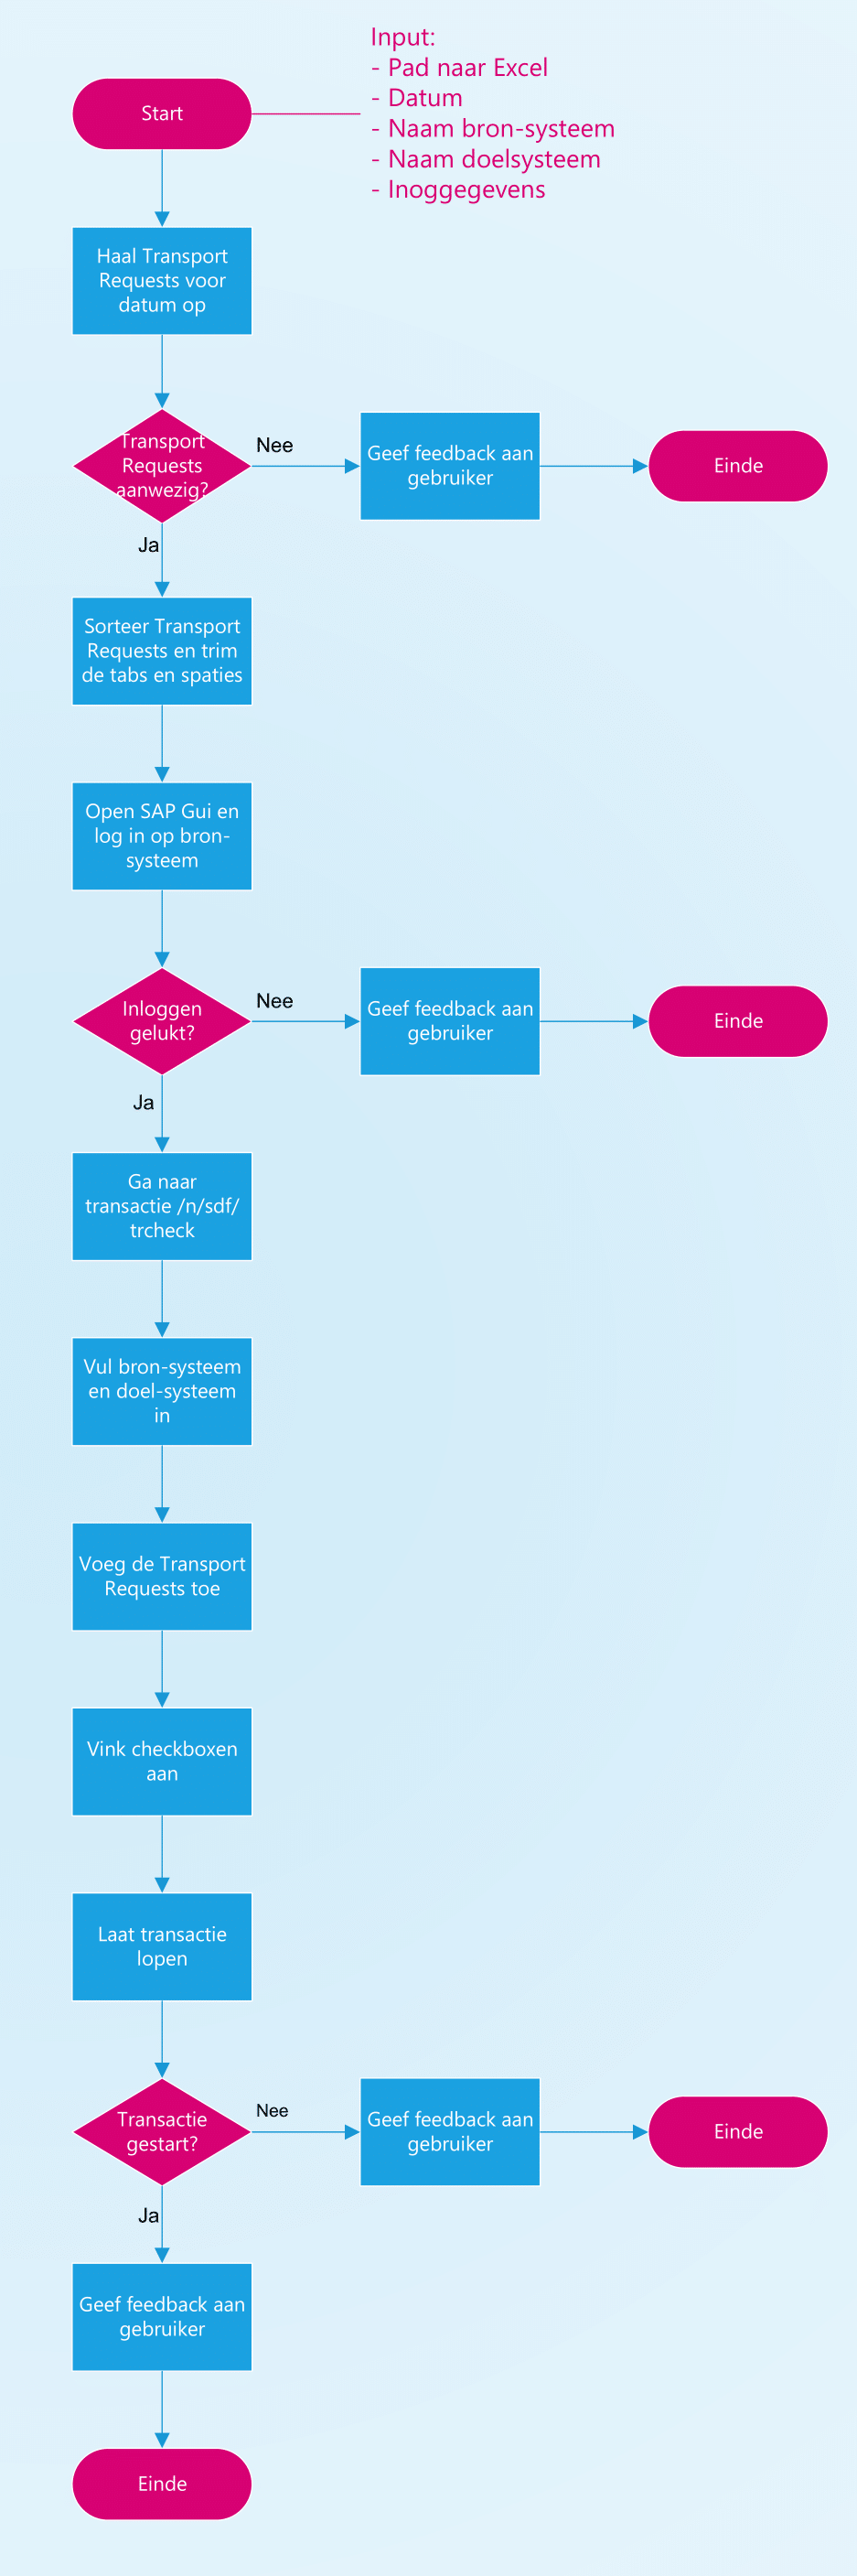
\includegraphics[width=0.5\textwidth]{../pictures/Flow_Cropped.png}
    \caption{Flow van het proces}
    \label{fig:flowchart}
\end{figure}
\label{fig:flowchart}

\subsection{Ontwikkeling van de Proof of Concept}
\label{subsec:ontwikkeling-proof-of-concept}

Het aanmaken van een RPA-automatisering via SAP BPA gebeurt in de BPA lobby. Op deze pagina worden alle eerder gecreëerde automatiseringen binnen het bedrijf getoond. Van hieruit wordt een nieuwe automatisering gecreëerd, waarna deze kan ontwikkeld worden binnen de BPA Process Editor. De process editor is de ontwikkelingsomgeving van SAP BPA.
Deze editor lijkt sterk op een flowchart-editor, wat logisch is als het seriële karakter van automatiseringsstappen bekeken wordt. De verschillende stappen worden één voor één gecreëerd en aan elkaar gelinkt. Hierbij kunnen variabelen worden doorgegeven en kunnen er verschillende condities zoals if-else-statements en loops geïmplementeerd worden.
Hieronder bespreken we kort de gecreëerde automatisering met de verschillende stappen.

\subsubsection{Start-formulier}
\label{subsubsec:start-formulier}

Zoals in de flowchart, die uit de design fase is ontstaan te zien is, heeft de automatisering verschillende input parameters nodig om de voorgestelde taken uit te kunnen voeren. Via de form te zien op afbeelding \ref{fig:startup-formulier} kunnen deze door de gebruiker opgegeven worden en kunnen deze gebruikt worden binnen de automatisering.
De verschillende waardes die opgegeven moeten worden zijn:

\begin{itemize}
    \item ExcelPad: het relatieve pad op het systeem van de gebruiker waar het Excel-bestand met de Transport Requests zich bevindt.
    \item Datum: de datum waarop de Transport Requests gefilterd moeten worden.
    \item BronSysteem: de naam van het systeem vanwaar de Transport Requests komen.
    \item DoelSysteem: de naam van het systeem naar waar de Transport Requests moeten overgezet worden.
    \item Gebruikersnaam: de gebruikersnaam van de gebruiker.
    \item Wachtwoord: het wachtwoord van de gebruiker.
    \item SysteemNaam: de connectie-naam waaronder het SAP-systeem is opgeslaan.
\end{itemize}

\begin{figure}
    \centering
    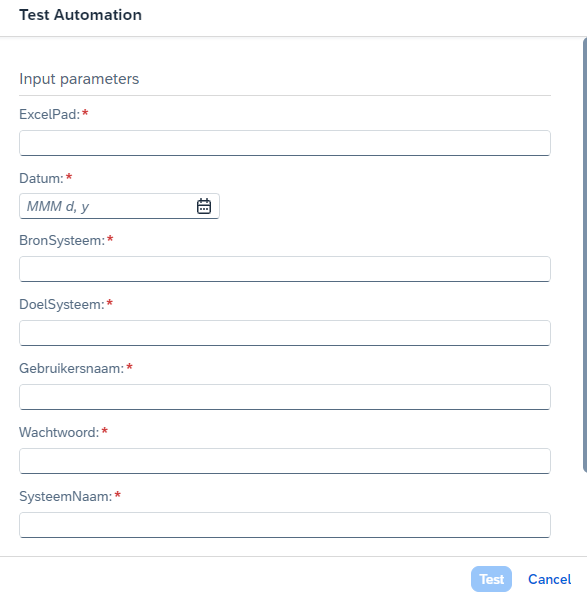
\includegraphics[width=0.8\textwidth]{../pictures/Startup_Form.png}
    \caption{Het start-formulier van de automatisering}
    \label{fig:startup-formulier}
\end{figure}

\subsubsection{Uitlezen van het Excel-bestand}
\label{subsubsec:uitlezen-excel}

De eerste grote stap die ondernomen wordt binnen de automatisering is het uitlezen van de Transport Requests uit het Excel-bestand. Hiervoor wordt het pad die de gebruiker bij de start heeft opgegeven, gebruikt om het Excel bestand te openen. Hierna kijkt de automatisering hoeveel lijnen het bestand kent, en via deze informatie haalt het alle informatie omtrent de Transport Requests uit het Excel-bestand via de Excel Cloud Link data-extractie taak.
Deze stappen zijn te zien op afbeelding \ref{fig:excel-lezen}.

\begin{figure}
    \centering
    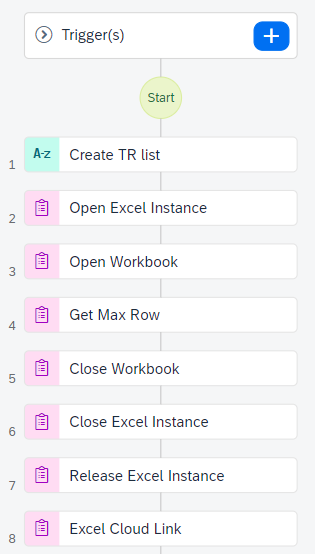
\includegraphics[width=0.8\textwidth]{../pictures/Read_Excel.png}
    \caption{Uitlezen van het Excel-bestand}
    \label{fig:excel-lezen}
\end{figure}

\subsubsection{Filteren van de Transport Requests}
\label{subsubsec:filteren-transport-requests}

Niet alle Transport Requests die in het Excel-bestand zijn opgeslagen moeten op hetzelfde moment overgezet worden. Via de datum die de gebruiker meegegeven heeft bij de start, worden de Transport Requests gefilterd. Enkel degene die op de opgegeven datum overgezet moeten worden worden aan de interne Transport Request lijst toegevoegd voor verdere verwerking.
Wanneer de Transport Requests gefilterd zijn en de te verwerken lijst is leeg, stopt de automatisering en wordt een melding gegeven aan de gebruiker.
Deze stappen zijn te zien op afbeelding \ref{fig:filter-transport-requests}.

\begin{figure}
    \centering
    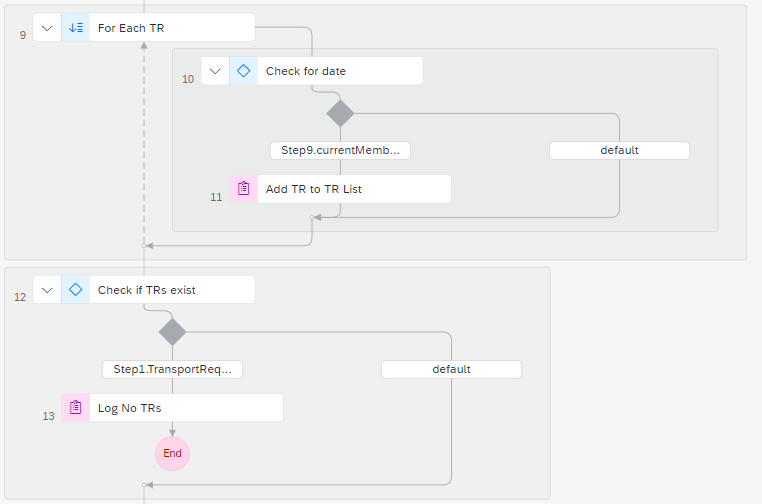
\includegraphics[width=0.8\textwidth]{../pictures/Check_Valable_TRs.png}
    \caption{Filteren van de Transport Requests}
    \label{fig:filter-transport-requests}
\end{figure}

\subsubsection{Inloggen bij SAP GUI}
\label{subsubsec:inloggen-sap-gui}

Nu de Transport Requests die gecontroleerd moeten worden gekend zijn, is het tijd voor de automatisering om zich in te loggen in de SAP GUI applicatie. Dit gebeurt in twee stappen. Eerst wordt de SAP GUI applicatie geopend en worden alle opgeslagen connecties opgehaald. De waardes van deze lijst worden dan één voor één vergeleken met de naam van het systeem die de gebruiker heeft meegegeven bij de start. Wanneer een connectie gevonden wordt die gelijk is aan deze meegegeven naam, wordt de positie in de lijst hiervan opgeslaan.
Deze stappen zijn te zien op afbeelding \ref{fig:controleren-connection-string}.

\begin{figure}
    \centering
    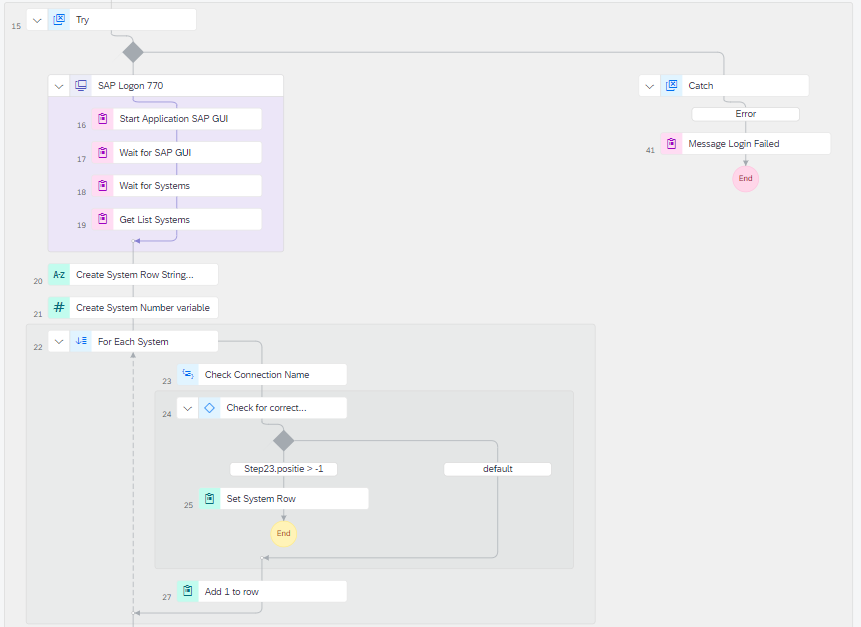
\includegraphics[width=0.8\textwidth]{../pictures/Check_Connection_String.png}
    \caption{Controleren van verschillende connecies}
    \label{fig:controleren-connection-string}
\end{figure}

Hierna wordt eerst gekeken of de connectie wel degelijk gevonden is. Wanneer dit niet het geval is wordt een melding getoond aan de gebruiker en stopt de automatisering.
Wanneer de connectie wel gevonden is, wordt deze via de berekende positie geopend en worden de inloggegevens van de gebruiker gebruikt om in te loggen binnen het systeem.
Deze stappen zijn te zien op afbeelding \ref{fig:inloggen-sap-gui}.

\begin{figure}
    \centering
    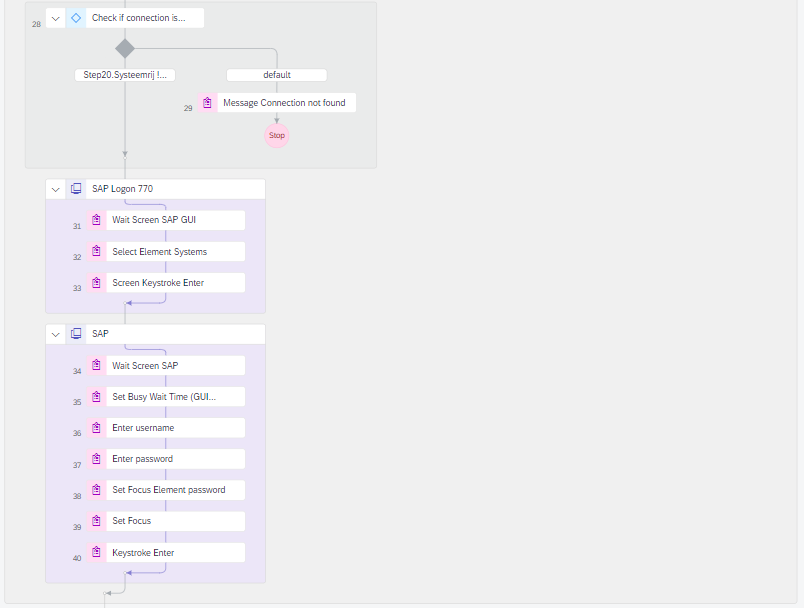
\includegraphics[width=0.8\textwidth]{../pictures/Login.png}
    \caption{Inloggen binnen SAP GUI}
    \label{fig:inloggen-sap-gui}
\end{figure}

Het volledige inlogproces staat binnen een try-catch block. Wanneer een stap zou falen, wordt er een bericht getoond aan de gebruiker en stopt de automatisering.

\subsubsection{Invullen van de de checken gegevens}
\label{subsubsec:invullen-checken-gegevens}

Nu de automatisering ingelogd is binnen het systeem kan de transactie om de Transport Requests te controleren geopend worden.
Wanneer deze geopend is worden zowel het bron-systeem als het doel-systeem ingevuld met de gegevens die de gebruiker bij de start van de automatisering heeft meegegeven.
Deze stappen zijn te zien op afbeelding \ref{fig:invullen-systemen}.

\begin{figure}
    \centering
    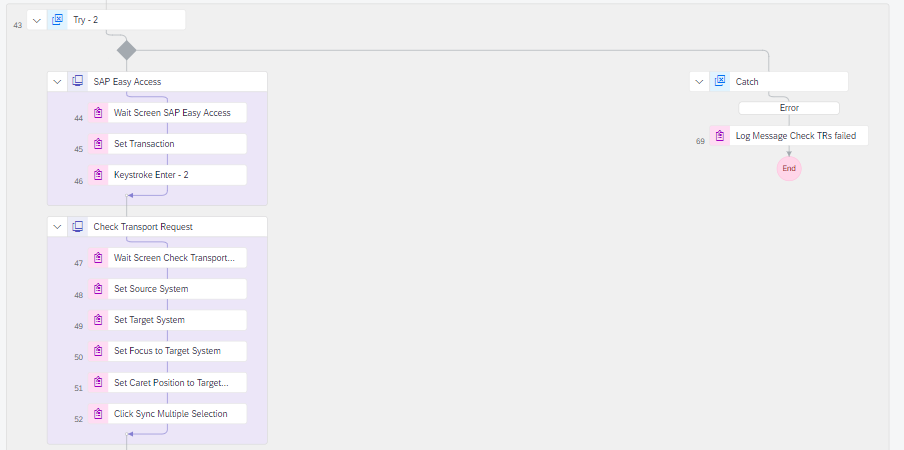
\includegraphics[width=0.8\textwidth]{../pictures/Set_Source_And_Target_System.png}
    \caption{Invullen van de systemen}
    \label{fig:invullen-systemen}
\end{figure}

Hierna wordt de lijst met gefilterde Transport Requests overlopen en worden ze ingevuld in de daartoe bestemde GUI tabel. Wanneer de volledige lijst ingevoegd is checkt de automatisering of de Transport Requests op een goede manier ingevuld zijn.
Deze stappen zijn te zien op afbeelding \ref{fig:controleren-transport-requests}.

\begin{figure}
    \centering
    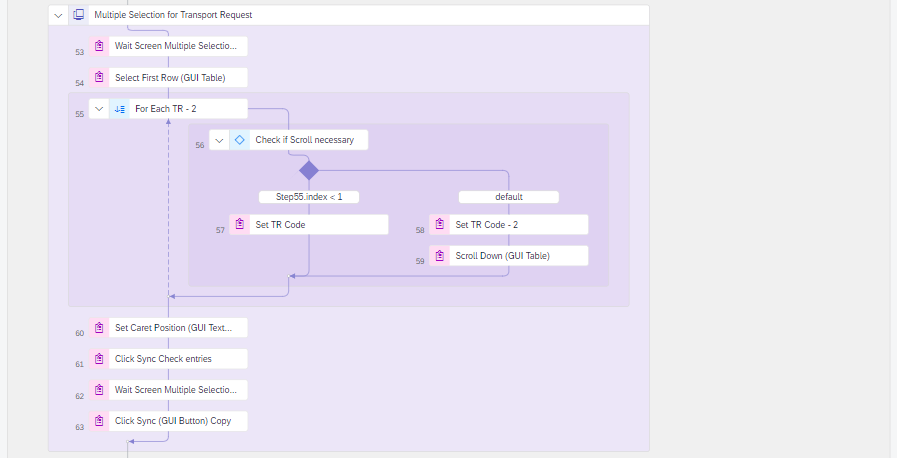
\includegraphics[width=0.8\textwidth]{../pictures/Enter_TRs.png}
    \caption{Invullen van de Transport Requests}
    \label{fig:controleren-transport-requests}
\end{figure}

Ook dit deel staat volledig binnen een try-catch block, dus wanneer de automatisering faalt wordt een melding getoond aan de gebruiker en stopt de automatisering.

\subsubsection{Controleren van de Transport Requests}
\label{subsubsec:controleren-transport-requests}

Nu alle gegevens ingevuld zijn vinkt de automatisering de checkboxes 'Cross Reference' en 'Sequence Check', de twee zaken die de automatisering moet controleren, aan. Hierna wordt de check gestart en geeft de automatisering het systeem terug aan de gebruiker. Wanneer de check voltooid is worden de resultaten van de check getoond en kan de gebruiker aan de slag met deze informatie.
Deze laatste stappen zijn te zien op afbeelding \ref{fig:controleren-trs}.

\begin{figure}
    \centering
    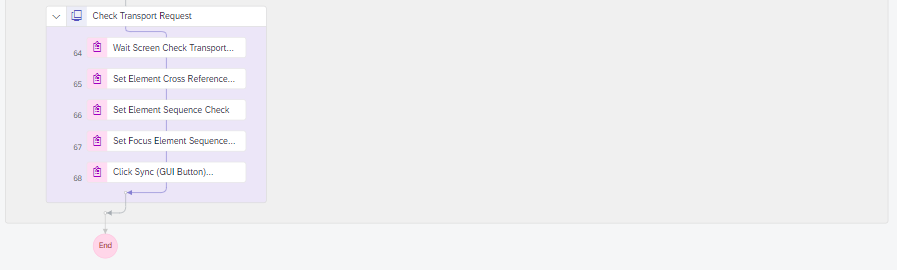
\includegraphics[width=0.8\textwidth]{../pictures/Checks.png}
    \caption{Controleren van de Transport Requests}
    \label{fig:controleren-trs}
\end{figure}

\subsection{Testen van de Proof of Concept}
\label{subsec:testen-proof-of-concept}

Wanneer de automatisering ontwikeld is, is het natuurlijk zeer belangrijk om deze te testen. Delaware heeft, als SAP-verdeler, een eigen testomgeving waarin mock-data beschikbaar is die een echt SAP-systeem nabootst. Dit is een uitgelezen manier om de automatisering te testen.
De automatisering werd een paar keer uitgevoerd en van dichtbij gemonitord om te zien of alle stappen wel degelijk op een goeie manier doorlopen werden. Ook werd het eindresultaat bekeken en getoetst aan de verwachtingen. De bot werd ook uitgevoerd met incorrecte gegevens, om te zien of het kan omgaan met uitzonderingen en deze op een correcte manier opvangt en rapporteert naar de gebruiker.

\section{Vergelijking met de huidige manier van werken}
\label{sec:vergelijking-huidige-manier}

Nu de Proof of Concept volledig uitgewerkt is, is het belangrijk om deze te vergelijken met de huidige manier van werken. Dit wordt op twee verschillende manieren gedaan. Als eerste wordt er gekeken naar de mogelijke tijdswinst die de automatisering oplevert.
Als tweede werd de consultant ondergevraagd over zijn mening over het gebruik van de automatisering. Hierbij wordt er gepolst naar of de automatisering het juiste proces uitvoert, de performantie en of het in zijn mening zijn werk zal vergemakkelijken.

\subsection{Tijdswinst}
\label{subsec:tijdswinst}

Om de tijdswinst van de automatisering te berekenen werd het proces 2 keer uitgevoerd door de betrokken consultant. De eerste keer werd het manueel uitgevoerd, zoals het nu dagelijks gebeurd. De tweede keer wordt de automatisering uit de Proof of Concept gebruikt.
Beide uitvoeringen werden getimed en de resultaten werden in tabel \ref{tab:tijdswinst} vergeleken.

\begin{table}[h]
    \centering
        \begin{tabular}{|l|l|}
            \hline
            & Tijd \\ \hline
            Manueel & 125,55 seconden \\ \hline
            RPA-automatisering & 24,39 seconden \\ \hline
            Tijdswinst & 101,16 seconden \\ \hline
        \end{tabular}
    \caption{Vergelijking van de duur van het proces met en zonder automatisering}
    \label{tab:tijdswinst}
\end{table}

Uit deze resultaten kan duidelijk afgeleid worden dat het proces duidelijk sneller uitgevoerd wordt via de automatisering. De automatisering werkt 5 keer sneller dan wanneer het manueel wordt uitgevoerd.
Wanneer dit proces dagelijks wordt uitgevoerd, kan deze automatisering over een lange tijdsperiode een zeer grote tijdswinst opleveren voor de consultant.

\subsection{Gebruiksgemak}
\label{subsec:gebruiksgemak}

Naast de tijdswinst is het voor nieuwe technologieën ook belangrijk dat de toekomstige gebruikers ook overtuigd zijn van de mogelijkheden ervan. Daarom werd de consultant, nadat hij de automatisering gebruikt had, ondervraagd naar zijn menig hierover.
Op de vraag of de automatisering het juiste proces uitvoert en het dit op een correcte manier uitvoert, antwoordde de consultant dat dit zeker het geval is. Ook merkte hij zelf op dat de automatisering in bijna elke stap sneller werkt dan hij de stap zou kunnen uitvoeren.
Op de vraag of hij de automatisering zou vertrouwen om deze taak uit te voeren, antwoordde hij dat dit niet direct het geval zou zijn. Zoals elke nieuwe tool zou hij de eerste dagen toch het resultaat een controleren en kijken of elk Transport Request wel degelijk meegegeven werd. Maar hij is ervan overtuigd dat er na een paar dagen zeker meer vertrouwen zal zijn in de automatisering en dat deze controle achterwege zal kunnen gelaten worden.
Op de laatste vraag, of hij denkt dat de automatisering zijn dagelijkse werk zal vergemakkelijken, antwoordde hij duidelijk ja. Hij gaf zelf aan dat, alhoewel het een vrij kort proces is, hij hier toch dagelijks tijd mee verliest en dit soms zeer frustrerend kan zijn, en deze automatisering hier een zeer grote hulp voor kan bieden.

Uit de antwoorden van de consultant kan duidelijk afgeleid worden dat hij zeer positief reageerde tegenover de automatisering en dat hij deze in de toekomst zeker zou gebruiken.